\chapter{Investigating Food Index-Based Food Diaries In The Lab}
\label{cha:cont2}
 
In this chapter, I explore challenges around self-monitoring dietary intake without a database on a mobile phone. In earlier chapters, I described the challenges and barriers that people face when employing a traditional approach to journaling what they eat, either on paper, a computer, or a mobile device. This project considers a different approach to the design of a food diary. Specifically, I begin to investigate how recording different information impacts the process of self-monitoring dietary intake. I defer to the constraints that a mobile platform imposes on the self-monitoring of intake problem as discussed earlier, and consider how the use of food indexes could address the given constraints. I also describe how the use of food indexes for mobile phone food journaling naturally reflects known guidelines for supporting successful goal-tending. After providing a theoretical grounding of the approach, I address practical concerns  of using food indexes for mobile phone food diary. I then describe a study where I explore some of those issues and present the results. 

\section{Introduction}
The BALANCE project highlighted the challenges of self-monitoring dietary intake on a mobile device. Many of the challenges were either directly or indirectly related to finding foods in a database. This led us to consider the problem of self-monitoring dietary intake without the database, believing this could help to streamline the food intake capture process. Tinker et al \cite{tinker_measurement_2001} discuss the potential benefits and drawbacks of ``brief'' self-monitoring instruments, pointing out three examples \citep{mossavar-rahmani_additional_2004,Roy1997, Mitchell1996} of previous work that compare the outcomes of brief survey versus detailed self-monitoring tools. \textit{Detailed survey} refers to food diaries that capture all details of an eating episode, including all foods, detailed serving sizes, and time of eating. They could also capture additional context such as location or other people. \textit{Brief survey} tools are designed to capture a fewer details of eating episodes. In the case of Tinker et al, the brief instrument was a `fat scan'. The fat scan is a single piece of paper designed to help users identify and monitor sources of fat in their diet. In addition to the paper-based instruments designed and evaluated above, Mattila et al \citep{mattila_mobile_2008} have used this brief approach to monitoring food intake on a mobile phone. However, this has not been compared to a detailed dietary intake monitoring tool. 

To inform the design of a new brief survey tool, we first considered the larger goal of the BALANCE project, which was to help people self-monitor their energy intake and expenditure to help either attain or maintain a certain weight. Self-monitoring is a tool to help support behavior change, in this case, around health and wellness behaviors. Self-monitoring helps people become aware of their current behavior. Continued self-monitoring helps to identify if the behavior is changing or not. This is related to goal setting and tending--- once awareness is developed via self-monitoring, one can begin to start defining targets for change. Defining goals raises the question of what kind of behavior change we can support without a food database.  A tool can not easily support calorie counting without a database for lookup. However, researchers are interested in other health and wellness indicators such as the quality of an individual diet. 

Diet quality is a factor in preventing and treating many diseases, such as cancer \citep{WHO_CVD_2011}, cardiovascular disease \citep{guh_incidence_2009}, and diabetes \citep{Hu2001}. Research has also shown that a diet high in nutrient dense food tends to be lower in calories \citep{Gibson2000, Cox2000}. Tools to support people in improving their diet quality, especially by increasing the amount of nutrient dense foods they consume, can help them to decrease the number of calories they consume. 

Diet quality is usually measured as a reflection of the pattern of food that an individual consumes, as opposed to values of specific nutrients \citep{kant_indexes_1996, kourlaba_dietary_2009,panagiotakos_adherence_2007}. Different patterns reflect different values of food pattern quality. For example, two dietary patterns commonly referred to include the Standard American Diet (SAD), which reflects how many Americans eat, and the Mediterranean dietary pattern (MedDiet), which reflects traditional eating practices in the Mediterranean. Diet quality is measured and evaluated is through the use of a food index. Food indexes usually consist of a number of components that are scored and then combined together to one overall score. Improving any of the component scores improves the overall score. Food indexes are thoroughly evaluated to ensure that they accurately represent a given diet. Further research investigates the correlation between a given food index and incidence of disease. 

Traditionally, food indexes have been used by experts to evaluate the diet quality of an overall population. Researchers take a form of food intake records (e.g. 24-hr recall, food frequency questionnaire), then calculate the components and overall score according to a set of rules. The report of the food index scores can be used to compare different populations (for example, men versus women in a particular geographic area), compare the change in diet quality over time, or identify areas where certain populations can improve their dietary intake. 

In the absence of a database, food indexes could be a good tool for individuals to track their dietary intake. However, food indexes were developed to be used by experts, and it is unclear what difficulties individuals will have in using them to characterize real food. 

In this chapter, I address the questions of how individuals can use food indexes to directly track their dietary pattern and quality, if there is a benefit in terms of reduced time to make an entry, how correct entries are, and if there is any perceived benefit to the users. 

\section{Food Indexes: Analyzing Diet Quality}
Dietary or food indexes are designed to describe the quality of the diet that a person or population consumes. An index has multiple components, which are weighted and scored differently, then combined to result in one overall number that describes an individual's diet. Research in the nutrition, epidemiological and medical fields correlate the value of different indexes to health outcomes, such as reduced incidence of cardiovascular disease, cancer, or simply mortality \citep{kant_dietary_2010,kant_dietary_2004,kuczmarski_higher_2010}. This makes them appropriate for consideration as a tool to support disease prevention. 

Traditionally, food indexes are used to understand the diet quality of a population as opposed to an individual. An index definition is usually comprised of multiple components and target consumption amounts. Components are either to be moderated (e.g., to place an improved score on consuming less) or attained (e.g., to eat at least a certain amount). Components are based on food groups (fruits, vegetables, grains) or nutrients (sodium, fat, protein) \citep{arvaniti_healthy_2008}. 
There are three basic groups of indexes, based on how they are created: those based on recommended dietary intake of micro- and macro-nutrients (calories, fat, protein, Vitamin A, sodium, fiber), an idealized or preferred dietary pattern (such as the Mediterranean diet), and food groups. An index based on recommended dietary intake uses nutrition databases to determine the macro-and micro-nutrients in each food eaten, and then generates a score via a formula. Indexes or scores based on an idealized pattern focuses more on the kinds of decisions people make about what they eat: choosing lean meats over fatty meats, and olive oil in place of butter. Finally, indexes based on food groups count how many servings of each food group is consumed. Overall, food indexes are discriminate between a diet full of nutrient dense foods and diets high in calorie-dense, nutrient-poor foods. 

An index is used by taking a traditional food journal that consists of a specific food eaten. For discussion purposes, I will refer to a cheeseburger as the specific food.  The researcher will code the food in terms of the food index components. With a food group-based index, the cheeseburger might be coded as ``2 servings of grains (the bun), 1 serving of meat (the patty), 1 dairy serving (the cheese)''. Once the coding is done, an overall score is generated based on a formula accounting for how each component should fit into the larger diet. Scores are sometimes averaged together over populations, which allows researchers to more easily compare or summarize food intake of a large number of people. 

For the purposes of this study, we have identified food indexes that are representative of the different types of food indexes. They are the Healthy Eating Index-2005 (HEI) \citep{guenther_development_2008, guenther_evaluation_2008} and the Food Based Quality Index (FBQI) \citep{lowik_food-based_1999}. The HEI is based on food groups and nutrient amounts, while the FBQI is based only on food groups. We felt it important to choose two indexes that embodied these characteristics for the purposes of exploring how these types of indexes appeal to users. We are choosing to not use an index based on the Mediterranean diet. An index based on an idealized dietary pattern assumes that the user has previously committed to a particular diet philosophy. 

\subsection{Food Indexes and Goal Setting}
\citep{consolvo_goal-setting_2009, cullen_using_2001,dewalt_goal_2009,intille_just--time_2003,locke_building_2002,shilts_goal_2004}

\subsection{The Healthy Eating Index-2005 }
The Healthy Eating Index (HEI) \citep{guenther_development_2008, guenther_evaluation_2008, kennedy_healthy_1995} is a food index based on the USDA Dietary Guidelines for Americans \citep{us_health_and_human_services_dietary_2005}. The original HEI was developed in 1995 and revised in 2006 to reflect the 2005 Dietary Guidelines. Throughout the rest of this document, the acronym `HEI' refers to the 2005 version of the HEI. 

The HEI is a score based system, with a high quality diet obtaining a score of 100 points. Each of 12 components contribute to the overall score. Table \ref{tab:table2_1} lists the components and their individual contribution to the overall score. The components above the line are attainment components. Researchers want people to eat more of these components. The attainment components for HEI contain primarily food groups. Components below the line are moderation components. Researchers recommend reducing or restricting the consumption of these components. All of these components are considered nutrients. The scoring of the attainment and moderation components reflect that most Americans do not eat enough of certain food groups (dark green and orange vegetables, whole grains) and consume too much of certain nutrients (sugar, saturated fat, calories). The calculation for each point depends on the individual daily recommended caloric intake.

% Table generated by Excel2LaTeX from sheet 'Sheet3'
\begin{table}[tbhp]
  \centering
  \caption[HEI Calculation.]{The HEI calculation. A close-to-perfect diet will score 100 points. Points are defined in regards to the recommended number of calories an individual should consume. Components above the line are attainment. Components below the line are moderation.}
    \begin{tabular}{p{2in}cl}
    \toprule
    \textbf{Component} & \textbf{Maximum Points} & \textbf{Daily Recommended Intake} \\
    \midrule
    Total Grains & 5     & $\ge$ 3.0 oz eq/1000 kcal \\
    Whole Grains & 5     & $\ge$ 1.5 oz eq/1000 kcal \\
    Vegetables & 5     & $\ge$ 1.1 cup eq/1000 kcal \\
    Dark green \& orange vegetables, legumes & 5     & $\ge$ 0.4 cup eq/1000 kcal \\
    Total Fruits & 5     & $\ge$ 0.8 cup eq/1000 kcal \\
    Whole Fruits & 5     & $\ge$ 0.4 cup eq/1000 kcal \\
    Milk  & 10    & $\ge$ 1.3 cup eq/1000 kcal \\
    Meat and Beans & 10    & $\ge$ 2.5 oz eq/1000 kcal \\
    Oils  & 10    & $\ge $12 g eq/1000 kcal \\
\hline
    Saturated Fat & 10    &$ \le 7\%  $ of total kcals consumed\\
    Sodium & 10    & $\le $0.7 g/1000 kcal \\
    Calories from Solid Fats, Alcoholic Beverages, and Added Sugars & 20    &   $\le$ 20\% of total kcals consumed \\
\hline\hline
    Total Points & 100   &   \\
    \bottomrule
    \end{tabular}%
  \label{tab:table2_1}%
\end{table}%


Grains, vegetables and fruits are broken into multiple categories. The grains category is separated into Whole and Total grains, as is the Fruit category. For Grains, once the daily limit is met for Whole Grains, more Whole Grains are counted under Total Grains. If a person eats five Whole Grains and five Total Grains, the grains component of the total score is 10. However, if a person eats 10 Total Grains, the grains component of the total score is 5, since none were Whole Grains and the max Total Grains score is 5. This is similar with Fruit, where Whole Fruits include unprocessed fruits, while Total Fruits includes juices and cooked or dried fruits. Vegetables also include two categories, separating out the dark green and orange vegetables, as well as legumes. Similar to Grains and Fruits, if one eats the equivalent of 10 points of Dark Green Vegetables, the total score is 10, while 10 points of other vegetables only contributes 5 points to the total score. 

The rules to calculate an HEI score for an individual diet are fairly complicated. However, partly due to the complexity, researchers find the resulting score a fairly good indicator of one's diet \citep{guenther_evaluation_2008}. The complexity makes it a good option for this study. It will help us to identify user responses to a complex interface and counting process. It also incorporates the restricting some important quantities. 


\subsection{The Food-Based Quality Index}
The Food-Based Quality Index (FBQI) \citep{lowik_food-based_1999} is a food index based solely on food groups. The FBQI food groups are simplified and slightly different than the ones based on the food groups defined by the USDA. Specifically, potatoes, rice, pasta, and other starchy grains are considered separately from either bread (and cereal grains) or vegetables. Cheese is separate from dairy. Serving specifications are designed to be representative of how consumers think about food servings. 

The FBQI is simpler than the HEI: It is based only on food groups with no accounting of nutrients; all components are target rather than attain or moderate; and serving sizes are intended to be user-friendly. However, the familiar serving sizes are vague. The simplicity of the FBQI is a good contrast to the HEI for an initial investigation of using food indexes for self-monitoring dietary intake. 

% Table generated by Excel2LaTeX from sheet 'Sheet4'
\begin{table}[tbhp]
  \centering
  \caption[FBQI Calculation]{FBQI Calculation. Each component accounts for a single point, but the target is a range. All components are targets; there are no attain or moderate components.}
    \begin{tabular}{lll}
    \toprule
    \textbf{Component} & \textbf{Points} & \textbf{Serving goal} \\
    \midrule
    Bread (incl. breakfast cereals) & 1     & 5-7 slices \\
    Potatoes (incl. rice, pasta \& pulses) & 1     & 3-5 pieces \\
    Vegetables & 1     & 3-4 serving spoons \\
    Fruit & 1     & 2 pieces \\
    Milk \& milk products & 1     & 2-3 glasses \\
    Cheese & 1     & 1-2 slices \\
    Meat, fish \& eggs & 1     & 115-130 g \\
    \bottomrule
    \end{tabular}%
  \label{tab:table2_2}%
\end{table}%

 
\section{Food Tasks: Food Diary Evaluation Methodology}
Section \ref{sec:food_task_challenges} details important considerations of choosing how to present food tasks to study participants. Those challenges are primarily how to choose which food to use in the tasks and how to present those foods to the participant. 

There are four options for presenting food tasks to participants: using real food; food models; food photographs; or food names. For practical purposes, we chose to use food names. For each food, the food name presented is from the Food Name field in the Nutritionist Pro KnowledgeBase. 

Food tasks were chosen... 
Concerns for choosing food tasks: 
\begin{itemize*}
\item Familiarity: chose foods from a previous study using the same population. 
\item combination foods: chose a balance of combo/prepared foods and single foods. 
\item amount of foods: used a 2000 kcal diet. 
\item number of foods: specific number of foods per meal. 
\item coverage for FBQI and HEI: chose foods to ensure that most or all components of HEI/FBQI were used in each `day' of food. 
\end{itemize*}


Since familiarity is so important, we carefully considered how to choose the food for the tasks. One considered approach was to refer to a published gold standard. [blah blah, not published, not an issue in nutrition research, etc. ] We considered using published diet plans, such as those advocated by the American Heart Association for healthy diets. The drawback to those is that they are recommended, and may not accurately reflect the actual diet of the participants. Additionally, since the recommended menus are based on the official Food Pyramid, and one chosen food index is also based on the Food Pyramid, this could influence the correctness scores. After consideration, we decided to choose the food tasks based on the food diaries collected in the BALANCE focus groups. Since the study populations are drawn from the same underlying populations, the issue of familiarity is addressed. More details are explained later. 

Another important aspect is how the food tasks are presented to participants. In the real world, one of the important challenges to ``perfect'' food journaling is the process of seeing/eating food, identifying what it is, sometimes identifying methods of preparation (fried versus broiled), identifying un-seen characteristics (low-fat versus full-fat milk, with butter), and identifying portion or serving sizes in order to correctly enter the food (or choose from a list in a db). Sometimes this process is easy, as with packaged foods or when preparing your own food; other times such as at a restaurant it is more challenging. Literacy is also an issue: with a traditional journaling approach, it is one thing to be able to identify one cup of spaghetti, but if you are not able to spell it properly, you might not be able to find it in a database. Due to this process, we considered that using real plates of food would be more life-like, and that using photographs of food were close to real. However, with the use of photographs, care must be taken to obtain them properly. Scale and lighting are two important considerations. And, with research, we found that there exist food photograph booklets specially prepared for the purpose of studying people's estimation of portion sizes. However, these booklets had the familiarity concerns outlined above. We decided that portion size estimation and literacy were not primary concerns for this study, so chose to present food tasks as a list of foods on a card. 

\section{Investigating and Comparing Food Index-Based Mobile Phone Food Diaries}
In this section, I talk about the evaluation I did to explore this area of tracking diet quality or food-index based tracking. 
\subsection{Research Aims}
\begin{enumerate*}
\item Is it faster to enter food in a complete, index-based mobile phone food diary?
\item Are people able to enter food correctly in a complete, index-based mobile phone food diary?
\item Are the work-load satisfaction measures the same for index-based mobile phone food diary as a traditional food diary?
\item How can we characterize the types of errors that are made in an index-based mobile phone food diary?

\end{enumerate*}

In addition to the above research questions, we designed this study to support generating design recommendations for future index-based food diaries. 

\subsection{Study Design}
We performed a comparative evaluation of the BALANCE interface with two food index-based food diaries. The other food diaries were based on HEI and FBQI. All interfaces were ran on a Windows Professional Mobile smartphone with a slide-out, qwerty keyboard. 

\subsection{Instruments}
This study focused primarily on understanding the interaction between people and a food index via a mobile device. 

The BALANCE interface was a modified version of the software for the BALANCE study. The modifications are detailed later. The HEI and FBQI interfaces were designed to be simple, similar, and reflect the food indexes. Both interfaces displayed all of the index components as boxes on the home screen. Daily progress for each component was shown as checks on each box. Each box had a button labeled ``Ex.''. This button opened a dialog window with a short description of the component and some example foods. This example information was intended to help users answer the question ``I just ate a food; which group does it go in?''. The example content was adapted from literature describing the indexes. 

Touching the index component button opens a serving size screen. This screen also provides examples of foods in that component and sample serving sizes. The widget for specifying servings was a set of buttons that could be toggled on and off. The buttons act like a slider: when a multiple-sized entry is made, all the others are selected. That is, clicking the 3 oz button selects the 1, 2, and 3 oz. buttons. 

The HEI and FBQI interfaces went through a paper prototype design process. One design feature explored in particular was the use of images to represent each component. Appropriate images could greatly improve user ability to remember what foods belong in which component. However, inappropriate images could have a large negative impact. Instead, we chose to use colors to represent each component. The same colors represented similar groups in HEI and FBQI, as much as possible. Finally, we designed the layout of the component buttons to all fit on the overview screen with no scrolling. This provided both an easy way to view the overview and make a new entry. 

Guiding Design Principles:
\begin{itemize*}
\item Overview on one screen
\item Overview shows progress but not goals or targets
\item Individual screens inherently showed goals (maximum number of boxes)
\item One handed use
\end{itemize*}


\subsubsection{HEI}
It is straightforward to convert the HEI index into a points-based system that is appropriate for our indexed-based system. For the study, we assumed a daily recommended intake of 2000 kcals. The official recommended intake for healthy adults is roughly 1900-2400 kcals/day. In real-world usage, the interface can reflect an individual's need, but for the study this was fine. We then calculated the recommended intakes for each group. For the interface, we made small adjustments to the amounts to target intakes to make it easier to count ``points''. We then chose a number of boxes to use to represent the points that was fairly straightforward and more human-friendly. For example, we rounded 2.2 cups of vegetables up to 2.5 cups, and presented it as 5 boxes, so that each box represented 0.5 cups of vegetables. This appears friendlier than 5 boxes with each representing 0.44 cups. We edited the ``What's in a serving'' text to reflect the amounts that each box represented. For the Vegetables, Fruits and Grains categories, where there are two sub-categories of foods, we ensured that each box for both sub-categories represented the same amount. For example, in the case of Grains, the target for Whole Grains is 3 oz, while the target for Total Grains is 6 oz. Rather than have 6 boxes for each (which means that the boxes for Whole Grains would represent 0.5 oz while the boxes for Total Grains would represent 1.0oz), we chose to have 3 boxes for Whole Grains and 6 boxes for Total Grains, and each box represents 1 oz. 

For the purposes of this study, we collapsed Fruit, Vegetables and Grains into single categories, each with two sub-categories. We did this to reduce the complexity of the overview screen for two reasons. First was because we wanted the overview screen to contain all of the index components and still be simple, uncluttered, and one-hand usable. Putting three more boxes on the overview screen would make the boxes too small. When the boxes are too small, they're more difficult to target/touch, and also have less space to show the checkmarks that identify current progress/status for the day. The second reason was that we wanted to reduce the cognitive load at the overview level. There are two tasks that we want to support with the overview screen: answering the questions of ``how is my progress so far today?'' and ``Where do I put this food?''. To answer the ``Where do I put this food?'' question, the fewer number of answers that are possible makes it an easier question to answer. For that immediate moment, it is easier (and quicker) for a person to judge ``is this carrot a fruit or a vegetable?''; once they get to the servings dialog, they can address the ``is it orange or not?'' question. 

% Table generated by Excel2LaTeX from sheet 'Sheet3'
\begin{table}[htbp]
  \centering
  \caption{Counting HEI as `tokens'}
    \begin{tabular}{p{2in}lllrl}
    \toprule
    Component & Goal  &       & Num Boxes & Daily Recommended Intake &  \\
    \midrule
    Total Grains & 6 oz  & 6 oz  & 6     & $\ge 3.0 oz eq/1000kcal$ &  \\
    Whole Grains & 3 oz  & 3 oz  & 3     & $\ge 1.5 oz eq/1000kcal$ &  \\
    Vegetables & 2.2 cups & 2.5 cups & 5     & $\ge 1.1 cup eq/1000kcal$ &  \\
    Dark green \& orange vegetables, legumes & 0.8 cups & 1 cup & 2     
& $\ge 0.4 cup eq/1000kcal$ &  \\
    Total Fruits & 1.6 cups & 1.5 cups &       & $\ge 0.8 cup eq/1000kcal$ &  \\
    Whole Fruits & 0.8 cups & 1 cup &       & $\ge 0.4 cup eq/1000kcal$ &  \\
    Milk  & 2.6 cups &       &       & $\ge 1.3 cup eq/1000kcal$ &  \\
    Meat and Beans & 5 oz  & 5 oz  & 5     & $\ge 2.5 oz eq/1000kcal$ &  \\
    Oils  & 24 g  & 25 g  & 5     & $\ge 12 g eq/1000kcal$ &  \\
    Saturated Fat &       & 7.5g  & 5     & $\le 7\%  of energy$ &  \\
    Sodium & 1.4 g &       &       & $\le 0.7 g/1000kcal$ &  \\
    Calories from Solid Fats, Alcoholic Beverages, and Added Sugars &   !!    &       &   !!?    & $\le 20\% of energy$ &  \\
    \bottomrule
    \end{tabular}%
  \label{tab:table2_3}%
\end{table}%



\begin{figure}	
\centering
	\begin{subfigure}[t]{1.25in}
		\centering
		\setlength\fboxsep{0pt}
\setlength\fboxrule{0.5pt}
\fbox{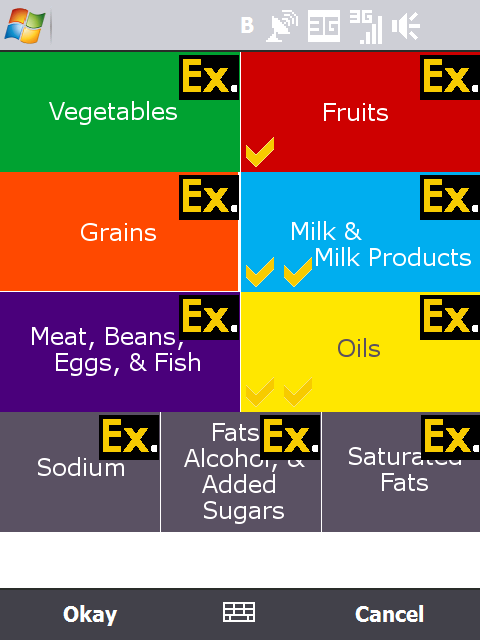
\includegraphics[width=1.25in]{./images/cont2/fig1a}}
		\caption{The main screen. Each block represents an HEI component. }\label{fig:hei_a}
	\end{subfigure}
\quad
\begin{subfigure}[t]{1.25in}
		\centering
		\setlength\fboxsep{0pt}
\setlength\fboxrule{0.5pt}
\fbox{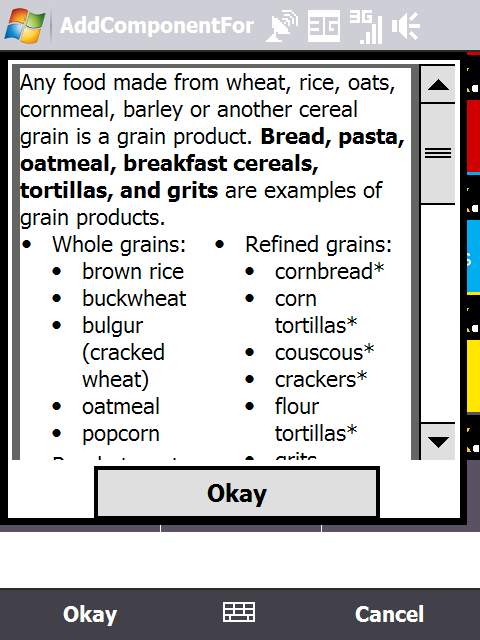
\includegraphics[width=1.25in]{./images/cont2/fig1b}}
		\caption{The `Ex.' button provides guidance on each component.}\label{fig:hei_b}
	\end{subfigure}
\quad
\begin{subfigure}[t]{1.25in}
		\centering
		\setlength\fboxsep{0pt}
\setlength\fboxrule{0.5pt}
\fbox{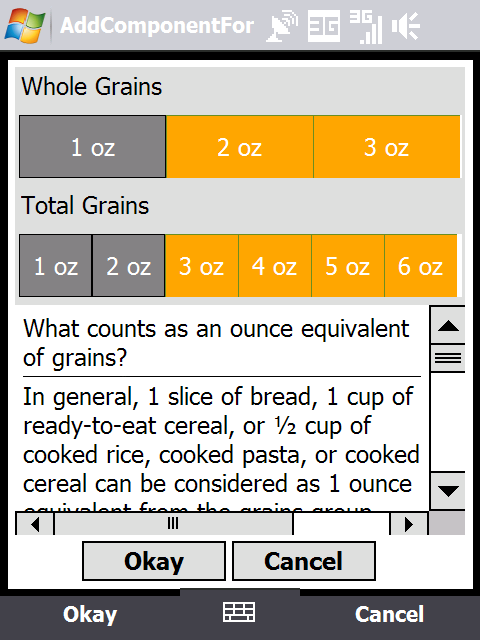
\includegraphics[width=1.25in]{./images/cont2/fig1c}}
		\caption{Touching a colored component box on the main screen opens a dialog where the user can specify how much of that component was eaten. One block represents a yellow checkmark.  }\label{fig:hei_c}
	\end{subfigure}
\quad
\begin{subfigure}[t]{1.25in}
		\centering
		\setlength\fboxsep{0pt}
\setlength\fboxrule{0.5pt}
\fbox{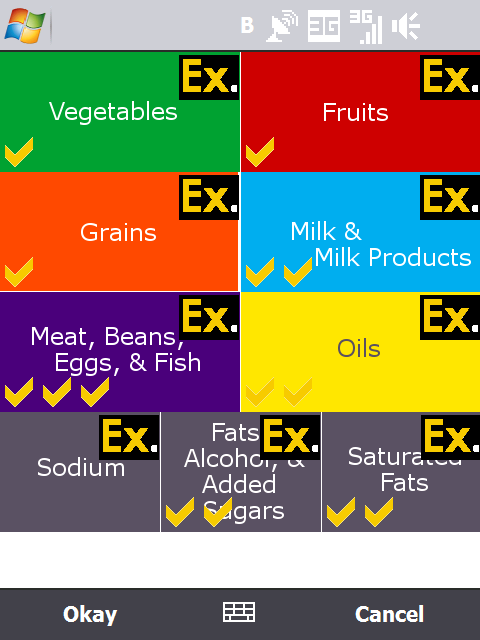
\includegraphics[width=1.25in]{./images/cont2/fig1d}}
		\caption{The yellow checks represent how much of each component was eaten on the current day. }\label{fig:hei_d}
	\end{subfigure}
	\caption{The HEI interface.}\label{fig:hei_instrument}
\end{figure}



The main screen of this application shows an overview of the index. Each colored button represents a component of the index, labeled as such. An ``Ex'' button on each component button provides support for the user to determine which group/component a particular food belongs to. The ``Ex'' button for Grains is shown above. With HEI, many of the components(Vegetables, Fruits and Grains) are broken down into sub-components. Once a component button is selected, a window pops up which allows a user to specify how many servings they  want to enter. Again, the example/explanatory information is presented on this page, to support the user in determining how many servings to select. For this study, the serving sizes was based on the formal HEI specification. We see in the case of grains, this is ounces of grains. The examples and explanatory guidance text is adapted from information provided by official food pyramid guidance. After the servings are selected, the overview screen shows checkmarks to represent the number of servings eaten in that category, accumulated for the day. 

\subsubsection{FBQI}

The FBQI interface is similar in design to the HEI inteface. This is specifically to attempt to minimize differences between the interfaces. As in HEI, the main screen shows an overview of the index. Each colored button represents a component of the index, labeled as such. An ``Ex'' button on each component button provides support for the user to determine which component a particular food belongs to. The ``Ex'' button for Grains is shown above. Once a component button is selected, a window pops up which allows a user to specify how many servings they  want to enter. Again, the explanatory information is presented on this page, to support the user in determining how many servings to select. The serving sizes and guidance are based on the official definition of the food index. The guidance for the FBQI is more streamlined, which is indicative of the point that the index is designed for experts, as opposed to novices. Consumers may find the simplification beneficial, but sometimes does not provide enough guidance for the various foods people encounter in their diet. The examples and explanatory guidance text is very similar to the guidance provided for HEI, and adapted from USDA food pyramid \citep{us_health_and_human_services_dietary_2005} guidance. After the servings are selected, the overview screen shows checkmarks to represent the number of servings eaten in that category, accumulated for the day. 

\begin{figure}	[tbh]
\centering
	\begin{subfigure}[t]{1.25in}
		\centering
		\setlength\fboxsep{0pt}
\setlength\fboxrule{0.5pt}
\fbox{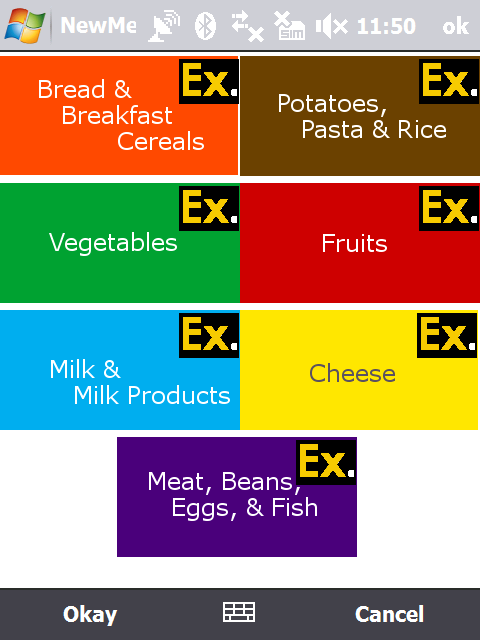
\includegraphics[width=1.25in]{./images/cont2/fig2a}}
		\caption{The main screen shows a colored box representing each component.  }\label{fig:fbqi_a}
	\end{subfigure}
\quad
\begin{subfigure}[t]{1.25in}
		\centering
		\setlength\fboxsep{0pt}
\setlength\fboxrule{0.5pt}
\fbox{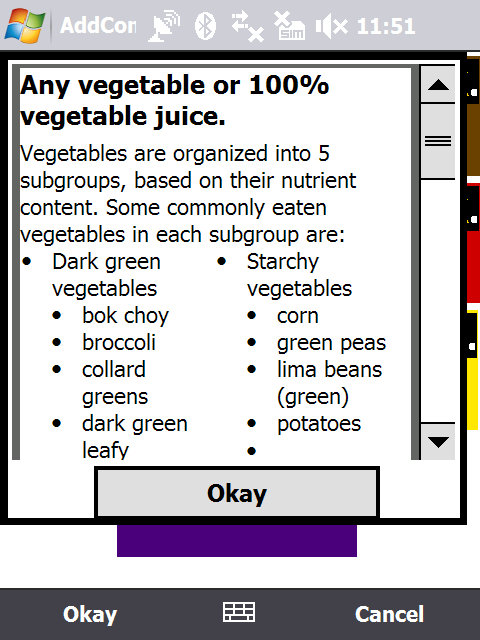
\includegraphics[width=1.25in]{./images/cont2/fig2b}}
		\caption{The `Ex.' button shows guidance for each component.}\label{fig:fbqi_b}
	\end{subfigure}
\quad
\begin{subfigure}[t]{1.25in}
		\centering
		\setlength\fboxsep{0pt}
\setlength\fboxrule{0.5pt}
\fbox{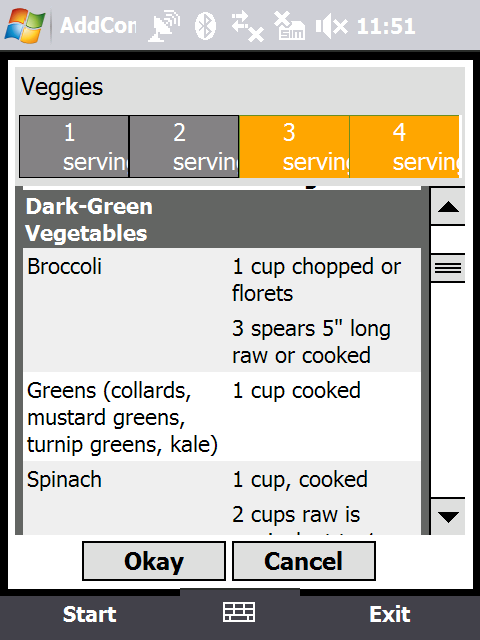
\includegraphics[width=1.25in]{./images/cont2/fig2c}}
		\caption{Touching the colored box opens a dialog where the user can specify how much was eaten. }\label{fig:fbqi_c}
	\end{subfigure}
\quad
\begin{subfigure}[t]{1.25in}
		\centering
		\setlength\fboxsep{0pt}
\setlength\fboxrule{0.5pt}
\fbox{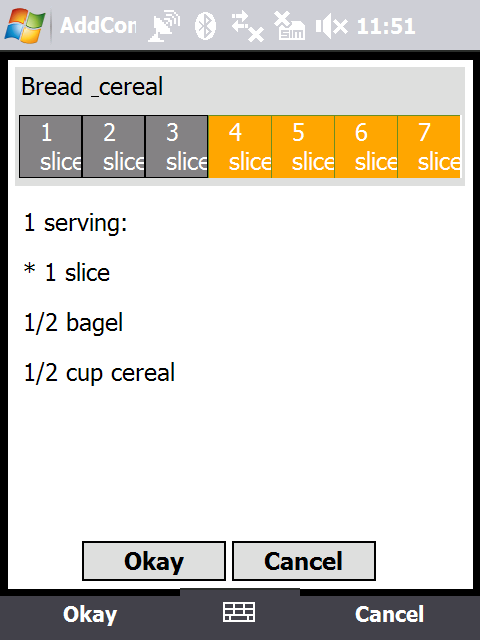
\includegraphics[width=1.25in]{./images/cont2/fig2d}}
		\caption{Yellow checkmarks show how much of each component had been eaten on the current day. }\label{fig:fbqi_d}
	\end{subfigure}
	\caption{The FBQI Interface. }\label{fig:fbqi_interface}
\end{figure}



\subsubsection{BALANCE}
The main, overview screen for the BALANCE software consists of a list of food eaten that day. For each food item, the name, number of calories, and meal is identified. The number of calories for that day is specified at the top of the screen. New entries are added by searching for a key word or name. After 3 letters are entered, a list is displayed that shows food entries (from a list of foods that contain common foods and foods that have been entered by that user before) that contain words starting the same way. After a specific food is chosen, a screen appears where the user can specify the amount eaten, in full and partial servings. Some foods provide multiple serving choices, such as ounces, cups, grams, pieces, or servings. This information is provided by the nutrition database, and is limited to the serving information in this database. 

\begin{figure}	[tbh]
\centering
	\begin{subfigure}[t]{1.25in}
		\centering
		\setlength\fboxsep{0pt}
\setlength\fboxrule{0.5pt}
\fbox{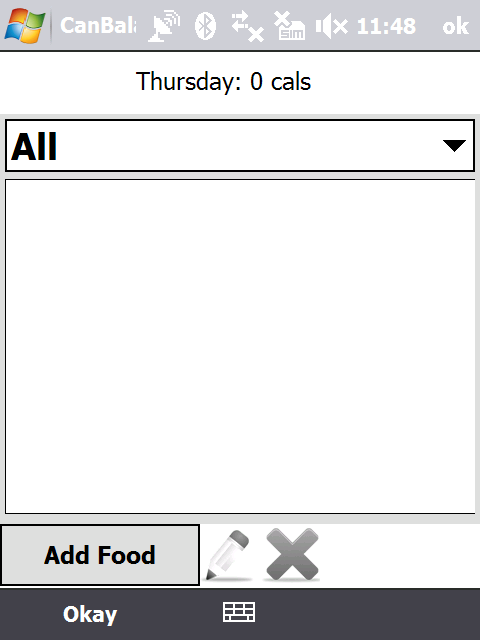
\includegraphics[width=1.25in]{./images/cont2/fig3a}}
		\caption{The modified BALANCE interface. The ``Add Food'' menu was changed to a button. The tool bar only allows editing and deleting food entries. }\label{fig:bal_a}
	\end{subfigure}
\quad
\begin{subfigure}[t]{1.25in}
		\centering
		\setlength\fboxsep{0pt}
\setlength\fboxrule{0.5pt}
\fbox{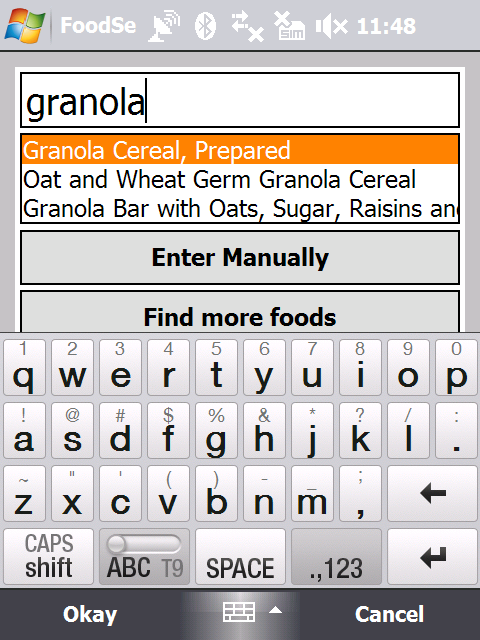
\includegraphics[width=1.25in]{./images/cont2/fig3b}}
		\caption{Enter the food name to search. }\label{fig:bal_b}
	\end{subfigure}
\quad
\begin{subfigure}[t]{1.25in}
		\centering
		\setlength\fboxsep{0pt}
\setlength\fboxrule{0.5pt}
\fbox{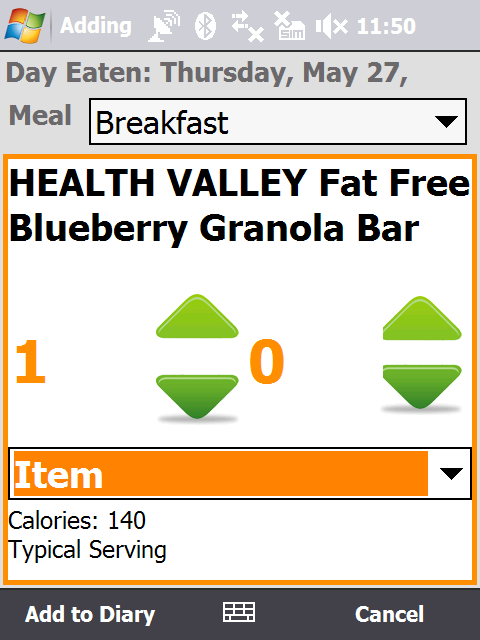
\includegraphics[width=1.25in]{./images/cont2/fig3c}}
		\caption{Specifying the amount eaten. }\label{fig:bal_c}
	\end{subfigure}
\quad
\begin{subfigure}[t]{1.25in}
		\centering
		\setlength\fboxsep{0pt}
\setlength\fboxrule{0.5pt}
\fbox{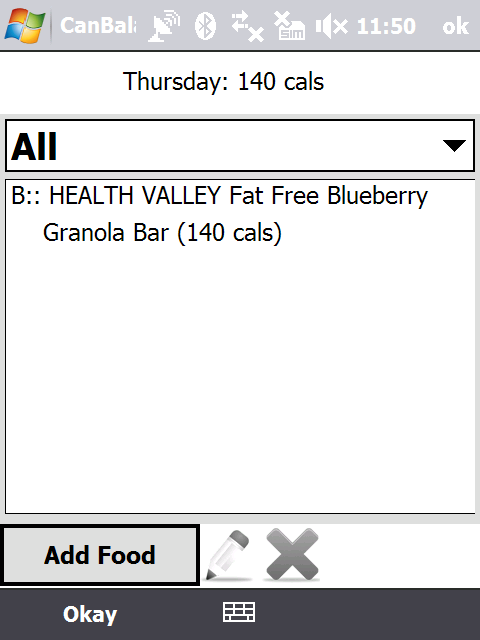
\includegraphics[width=1.25in]{./images/cont2/fig3d}}
		\caption{The food listed on the main screen. }\label{fig:bal_d}
	\end{subfigure}
	\caption{Modified BALANCE interface. }\label{fig:bal_interface}
\end{figure}



\subsection{Participants}

12 participants, recruited from online campus newspaper. The mean age was 31.6 years, median age 28.5 years; 8 females. 7 participants owned a phone with a touch screen, 5 owned ``feature phones''. Of the 12 subjects, 10 of them reported using their cell phone either daily (1-2 times per day) or several times a day, while 2 reported using their phones approximately 1-2 times per month. 7 reported entering text (such as text messages or adding/modifying contacts) on their phones either daily (1-2 times per day) or several times a day, while 3 enter text approximately 1-2 times per week and 2 almost never enter text on their phones. Of participants who enter text on their phones, 5 use a 12-key keypad; 3 use a touch screen or soft keyboard; and 3 use a QWERTY or hardware keyboard. 

\subsection{Procedure}
Participants came to the lab, and began by filling out a questionnaire that included basic demographic data, questions concerning the participants' daily cell phone use, current health and wellness goals, and experience journaling food intake. 

Then, for each interface, they were introduced to the interface and given two practice tasks to perform. The practice tasks were the same for all interfaces. One practice task consisted of only single foods, and the other practice task consisted of combination foods. After the practice tasks, the participants were given a chance to ask any questions or take a break. They were then notified that the real tasks were starting, and asked to work as quickly as comfortable between the start of a task and the end. 

A task consisted of a meal, which was printed on a card. At the start of each task, the task card was set on the table next to the participant, and phone displayed a screen that identified the coming task (by task ID). This allowed the study administrator to ensure that the correct task was being timed (by comparing the task ID on the screen with the card). When the participant is ready, they click on the ``Start Task'' button, then refer to the task card for entries. When the participant believes the task is complete, they click the ``done'' button. Another screen showed that the task was over. The participant then clicks ``next task'' when they are ready, and the cycle starts again. 
One day of meals was completed in each condition. This consisted of a breakfast, lunch, dinner, small snack, and large snack. After each condition, participants filled out a TLX survey and asked what they like best and least about each condition. The presentation of food days and order of conditions was counterbalanced.

After all three conditions were complete, the participants completed a final survey on the computer. 

\subsection{Tasks}
For each condition, participants have ``food tasks'' for the participants to enter. Food tasks are broken down into ``meals'', and there will be a controlled set of foods in each meal. 

There were 3 days of food tasks. Each day consisted of a breakfast (3 food items), small snack (1 item), lunch (4 items), big snack (2 items), and dinner (6 items). Each day was chosen to control for number of items, number of calories, and number of index components. Foods and meals were chosen from a previous study that collected food journals from a similar population. This ensured that most foods would be recognized and familiar. Specifically, foods were chosen only if they existed in the nutrition diary that BALANCE is based on. This has the benefit that we can more closely compare things like time to enter between conditions, but it is clearly not representative of the real world, where many foods are not included in the database. This is a problem that has proven to be a barrier for many food diaries. 

\subsection{Study Design Limitations}
This study simplifies the food journaling process in order to directly compare the strengths and weaknesses of the interfaces. There are three primary limitations to the design of this study: it does not address the problem of either estimating or measuring serving sizes; none of the tasks include foods that are not in the database; and there is no real-world context. 

\subsection{Data Collected}
The data collected is described in more detail below. Special attention is given to the treatment of how to count task responses as correct. 


\textbf{Duration.} Time spent in each condition. Time was calculated as the sum of time spent in each meal, starting when the ``start'' button was clicked and stopping when the ``done'' button was clicked at the end. Time between meal tasks was not counted. 



\textbf{Correctness.} A value indicating how correct the task response was. A task is assigned 2 points for entirely correct, 1 point for mostly correct, and 0 points for not correct. A participant can get a maximum score of 10 in each condition. Entirely correct means it is exactly ground truth; mostly correct means that there was a small difference that was not entirely correct, but the meaning was close (for example, replacing ``feta'' with ``blue cheese'', or ``Hidden Valley Ranch Dressing'' with ``creamy salad dressing'' in the BALANCE condition). This was done by inspection by the lead researcher. 

This approach to measuring correctness is due to the complexity of comparing errors across conditions. In all three conditions, it was common for users to provide an answer that was close to correct, but not entirely. This approach, in conjunction with a more thorough analysis of the exact errors that were made, allows us to better compare how well participants performed in each interface. 


\textbf{TLX.} Self-reported measure of workload assessment. After each condition, participants filled out a NASA-TLX survey \citep{Hart2006}. Items include Mental Demand, Physical Demand, Temporal Demand, Performance, Effort, and Frustration,  and are rated on a 7-point Likert scale. 

\textbf{Rankings.} Ordering of the interfaces on four features. At the end of the study, participants ranked each interface in terms of preference, ease of use, understandability, and usefulness.

\textbf{Useful for goals.} Self-reported indication of how useful each interface would be to help reach goals. At the end of the study, participants were asked which single interface they felt would be most helpful for them to reach their health and wellness goals, and why. 



\textbf{Length of use.} Self-reported duration a participant would be willing to use the interface for. At the end of the study, participants were asked which interfaces they felt they could use for three days, three weeks, and three months. 

\textbf{Likes and dislikes. } Self-reported features that participants liked or did not like. After each condition, participants were asked to list three things they liked about the previous condition, and three things they did not like.

\textbf{Errors.} Difference between the ideal or expected task response and what the user entered. An error was identified as a difference between a participant food entry (the final ``daily'' entry'') and the expected/perfect entry. This is different than the correctness measure described earlier. Correctness is a score designed to support comparison between conditions. Here, we compare and report on the errors within one condition. 


\subsection{Hypotheses}
Tested hypotheses: 
\begin{enumerate*}
\item Both of the index-based interfaces (HEI and FBQI) will be faster than the BALANCE interface. 
\item The FBQI interface will have more errors than the BALANCE interface; HEI interface will have more errors than the FBQI interface.  
\item The TLX workload measures will be the same for all three interfaces. 
\end{enumerate*}

Can we begin to characterize the types of errors that are made in a complete, index-based mobile phone food diary? 


\subsection{Data Analysis and Results}
Since this work was an early exploration, we performed both quantitative and qualitative analyses. The quantitative analysis focused on comparing performance of the interfaces. The qualitative analysis focused on proving insight into the use of the food indexes for self-monitoring of dietary intake. This included a thematic analysis of the answers provided to the self-report questions, an analysis of the errors made in each condition, and a discussion of the answers to the question ``Which interface will help you reach your health and wellness goals?''


% Table generated by Excel2LaTeX from sheet 'Sheet5'
\begin{table}[htbp]
\tiny
  \centering
  \caption{Summary of statistical analyses}
    \begin{tabular}{lp{1.5in}cp{2.5in}}
    \toprule
    Measure & Test  & Significance & Values to report \\
    \midrule
    \textbf{Correctness}\footnote[1]{Significant}
 & 1-way repeated measures ANOVA & Y     & ($F_{2,22}=17.074, p<0.0001$). \\
    \textbf{} & Paired t-test & Y     &  \\
    \textbf{Duration}$^{a}$ & 1-way repeated measures ANOVA & Y     & (Wilks� lambda $= 0.154, F_{2,10}=27.49, p<0.0001$). \\
    \textbf{} & Paired t-test & Y     &  \\
\midrule
    \textbf{TLX: } &       &       &  \\
    \multirow{2}[0]{*}{\textbf{Mental Demand}} & \multirow{2}[0]{*}{Friedman test} & \multirow{2}[0]{*}{Y} & \multirow{2}[0]{*}{ ($\chi^2=10.56, N=12, df=2, p<0.01$).} \\
          &       &       &  \\
    \textbf{} & Wilcoxon & N     & With Bonferroni correction, no pair-wise comparisons are significant.  \\
    \textbf{Discouraged} & Friedman & N     & ($\chi^2=2.595, N=12, df=2, p=0.273$). \\
    \multirow{2}[0]{*}{\textbf{Ease of use}} & \multirow{2}[0]{*}{Friedman} & \multirow{2}[0]{*}{N} & \multirow{2}[0]{*}{($\chi^2=3.556, N=12, df=2, p=0.169$).} \\
          &       &       &  \\
    \multirow{2}[0]{*}{\textbf{Quickly}} & \multirow{2}[0]{*}{Friedman} & \multirow{2}[0]{*}{N} & \multirow{2}[0]{*}{($\chi^2=1.333, N=12, df=2, p=0.513$).} \\
          &       &       &  \\
    \textbf{Learn} & Friedman & N     & ($\chi^2=0.963, N=12, df=2, p<0.618$). \\
    \multirow{2}[0]{*}{\textbf{Successful}$^{a}$} & \multirow{2}[0]{*}{Friedman} & \multirow{2}[0]{*}{Y} & \multirow{2}[0]{*}{ ($\chi^2=16.89, N=12, df=2, p<0.0001$).} \\
          &       &       &  \\
    \multirow{3}[0]{*}{\textbf{}} & \multirow{3}[0]{*}{Wilcoxon} & Y     & HEI vs BAL: ($z=-2.831, p<0.01$) \\
          &       & Y     & FBQI vs BAL: ($z=-2.825, p<0.01$) \\
          &       & N     & FBQI vs HEI: not significant \\
    \textbf{} &       &       &  \\
\midrule
    \textbf{Rankings} &       &       &  \\
    \multirow{2}[0]{*}{\textbf{Preference}} & \multirow{2}[0]{*}{$\chi^2$ test of proportions} & \multirow{2}[0]{*}{N} & \multirow{2}[0]{*}{($\chi^2=4.5, N=12, df=2, p=0.105$).} \\
          &       &       &  \\
    \textbf{Understandability}$^{a}$ & $\chi^2$ test of proportions & Y     & ($\chi^2=9.5, N=12, df=2, p<0.01$). \\
    \textbf{} & $\chi^2$ test of proportions: BAL vs FBQI & Y     & ($\chi^2=6.4, N=10, df=1, p<0.05$). \\
    \textbf{} & $\chi^2$ test of proportions: BAL vs FBQI & Y     & ($\chi^2=4.46, N=11, df=1, p<0.05$). \\
    \textbf{} & $\chi^2$ test of proportions: HEI vs FBQI & N     & ($\chi^2=0.333, N=3, df=1, p=0.564$). \\
    \textbf{Ease of Use} & $\chi^2$ test of proportions & N     & ($\chi^2=1.5, N=12, df=2, p=0.472$). \\
    \textbf{Usefulness} & $\chi^2$ test of proportions & N     & ($\chi^2=1.33, N=12, df=2, p=0.248$). \\
    \bottomrule
    \end{tabular}%
  \label{tab:table2_4}%
\end{table}%


\subsubsection{Duration}
Duration addresses Hypothesis 1: the HEI and FBQI interfaces are faster than the BAL interface. 

A single, categorical independent variable and a single, continuous, normally-distributed dependent variable. 
Since Mauchly's test is significant, we can use either the multivariate test or the univariate test with correction. 
A multivariate repeated measures ANOVA indicates that timing is significantly different with each interface (Wilks' $\Lambda = 0.154, F_{2,10}=27.49, p<0.0001$). 
In the univariate repeated measures ANOVA, Mauchly's sphericity test is significant ($\chi^2=8.127, N=12, df=2, p<0.05$). The Greenhouse-Geisser corrected test indicates that duration is significantly different with each interface ($F_{1.23,14.14}=21.115, p<0.0001$). 

All pairwise comparisons are significant using Holm's sequential Bonferroni procedure ($\alpha = 0.05$). We can accept our alternative hypothesis that HEI and FBQI are faster than BAL. FBQI is significantly faster than HEI. 


\subsubsection{Correctness}
The correctness measure addresses Hypothesis 2: the FBQI interface will have more errors than the BALANCE interface, and the HEI interface will have more errors than the FBQI interface. 
 
There is 1 categorical independent variable (interface) and 1 continuous dependent variable assumed to be normal. 

In the univariate repeated measures ANOVA, Mauchly's sphericity test is not significant ($\chi^2=1.351, N=12, df=2, p=0.509$). The results, assuming sphericity, indicates that timing is significantly different with each interface ($F_{2,22}=17.074, p<0.0001$). 

Pairwise comparisons using Holm's sequential Bonferroni procedure show that HEI is significantly less correct than FBQI ($p<0.017$) and BAL ($p<0.025$), but that FBQI is not significantly less correct than BAL. 

\subsubsection{TLX}
The TLX measures reflect user perception of workload and address Hypothesis 3. 

Each question is a single, categorical, multi-level independent variable and a single, continuous dependent variable. 

For each of the seven TLX ratings, we use the Friedman test to determine if there is a significant difference between each of the three interfaces. If the Friedman test has a significant result, we use Wilcoxon test on a pair-wise basis to identify which pairs are significant.

Only two TLX measures resulted in a significant Friedman test, Successful ($\chi^2=16.89, N=12, df=2, p<0.0001$) and Mental Activity ($\chi^2=10.56, N=12, df=2, p<0.01$). Follow up Wilcoxon tests (with Bonferroni correction) show that there are no significant pair-wise differences in Mental Activity.  For the Successful measure, HEI is significantly lower than BAL ($z=-2.831, p<0.01$), and FBQI is significantly lower than BAL ($z=-2.825, p<0.01$), but there is not a significant difference between FBQI and HEI. 

\subsubsection{Rankings}
Performed a 1-Sample $\chi^2$ test of proportions based on the \#1 rankings for each item, to determine if the distribution of \#1 rankings were significantly different than chance for each ranking item. The expected proportions are that each interface is ranked \#1 the 33% of the time for each ranking. The ?2 test of proportions tests if the observed proportions match the expected. 
Of the four rankings (preference, ease of use, understandability, and usefulness), only Understandability is significantly different than expected. Follow-up pair-wise $\chi^2$ testing revealed that significantly more people found BAL more understandable than FBQI ($\chi^2=6.4, N=10, df=1, p<0.05$), BAL more understandable than HEI ($\chi^2=4.46, N=11, df=1, p<0.05$), but not a significant difference between FBQI and HEI. 

While the $\chi^2$ test for usefulness did not have a significant result, it poses an interesting case as no one ranked FBQI as \#1 in usefulness. 

\subsubsection{Useful For Goals}
At the end of the study, participants were asked which interface they thought would help them reach their health and wellness goals. Participants only chose BAL or HEI as an answer to this question, hence FBQI is not shown below. The chart below presents the answers to this question, combined with responses to the question (asked at the beginning of the study) ``What are some of your health and fitness goals?''. This was a multiple choice question with a write-in option. 
 

\begin{figure}[ tbh ]
\begin{center}
\setlength\fboxsep{0pt}
\setlength\fboxrule{0.5pt}
\fbox{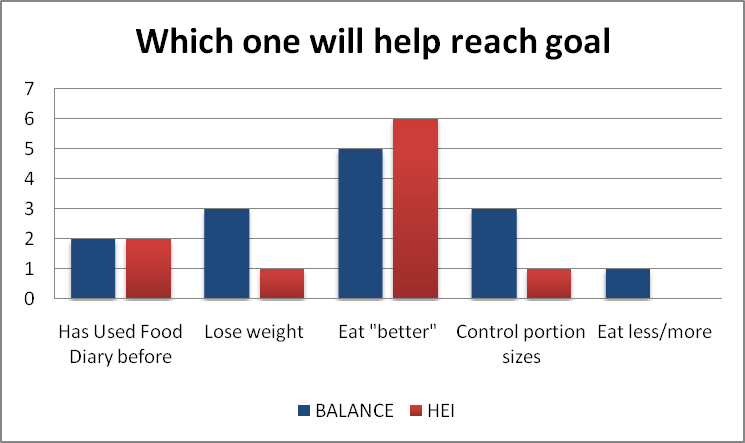
\includegraphics[ width=3.5in ]{./images/cont2/chart1}}

\caption{Answers to ``Which interface will help you reach your goals?''}
\end{center}
\end{figure}


Finally, we asked participants which one they thought would be most helpful in reaching their nutrition goals. The above chart shows the choice that participants made, separated out into the goals they reported at the start of the study. Participants selected BALANCE for the goals that depend more on quantitative data (losing weight which requires counting calories, controlling portion sizes, and eating less or more), which provides more detail. Participants selected HEI for goals that are more qualitative (eat ``better''). This led us to the question of whether one approach or the other reflects whether an individual's nutrition goal is quantitative or qualitative.

\subsubsection{Error Analysis}
In this section, I breakdown the errors participants made in BALANCE and FBQI. The process we used was to identify all items with errors, and then characterize them. 

\textbf{Most Challenging Tasks}
Here, we discuss the tasks that were most challenging for participants in the different conditions. No task in the BALANCE condition was entirely wrong (all scores are above 6), and as our correctness score above reports, the most errors were made with the HEI interface. 

\textbf{HEI. }
Using HEI, there were two tasks that no participant entered correctly. The first was a dinner consisting of spaghetti, peas, parmesan, garlic bread, green salad, Ranch dressing. The second was a snack that consisted only of Doritos. No one entirely correctly entered three tasks: a dinner (Meatloaf, mashed potatoes, lettuce salad, Thousand Island dressing, gravy, milk) and two breakfasts: (Bagel, cream cheese, latte) and (Breakfast burrito with eggs, bacon and cheese, apple juice, banana). The meatloaf dinner was also never correctly entered in  FBQI. 
 
\textbf{BALANCE. }
Participants made 23 errors in the BALANCE condition. One was due to a technology failure. The remaining 22 errors were executed by seven of the participants. The other five participants had no errors in this condition. Four people had 1 error, one person had 2 errors, one person had 7 errors, and one person had 9 errors.

There were two types of errors. First was a serving size error: the participant entered the wrong serving size. There were three instances of this error. All three instances consisted of the participant entering ``1.xx'' units (e.g., 1\textonehalf units) rather than ``xx'' units (e.g. \textonehalf units). We believe this is due to the participant not modifying the whole number part of the default amount presented in the interface, but only modifying the partial number part of the default amount. Two of the three people who had this kind of error made no other errors.

There were 19 instances of substitution error. A substitution error is defined as when the participant chose a similar food rather than the exact food. All of these errors were the result of choosing foods that are slightly different than the target food. Examples include ``Spinach leaves'' rather than ``Spinach Salad'', ``Iceburg Lettuce'' rather than ``Iceburg Lettuce Leaves'', generic ``Swiss Cheese'' rather than ``Pauly County Line � Swiss Cheese''. Most participants with this kind of error only had one substitution. Two participants had 7 and 9 substitutions, respectively. These two participants could represent a user profile of someone for whom ``close is good enough'' holds true. 

\textbf{FBQI. }
Participants made 24 errors in the FBQI condition. One participant did not have any errors. Individual participants had error counts that ranged from 1-4. Three participants had 1 error; four participants had 2 errors; three participants had 3 errors; and one participant had 4 errors. 

We identified four types of errors in FBQI: Over-counting (counting too many in the correct category), under-counting (counting too few in the correct category), miscategorizing (counting something that belonged in one category in a different one), and non-counting (an entire category is not counted).

There were three instances of mis-categorizing. In one case, a food that should be counted as a ``Bread'' was counted as a ``Potato'' (chocolate chip cookie). Once a ``Milk'' was counted as a ``Cheese'' (cream cheese or latte), and once a ``Cheese'' was counted as ``Milk'' (Swiss cheese).

There were three instances of under-counting. In these cases (B3, D3, B1), a category had one serving entered, rather than the expected two servings. The same participant counted a bagel as one bread serving, and a salad and broccoli as one vegetable serving rather than two. The last instance of under-counting was when a participant entered one serving to cover four apricots and granola with raisins.

There were 8 instances of over-counting. All of the over-counting errors were counting one more than expected.

There were 7 instances of non-counting:
\begin{itemize*}
\item No potatoes counted for `$2/3$ c. mashed potatoes'
\item No milk for `latte' (2 times)
\item No bread for `Wheat Thins'
\item No veggies for `peas' and `salad' (2 times)
\item No meat for `pepperoni'
\end{itemize*}


\subsubsection{Likes/Dislikes}
After completing each condition, participants were asked to list three things they liked and three things they did not like about each interface. Responses were free form. The lead researcher clustered the response. The process used was to: read through all items; identify clusters or group topics for each condition; attempted to identify similar clusters across conditions; put the raw items into the groups; collapse very similar items into a single item; count the instances of each item and each group. Because of the different nature of the index-based interfaces (HEI and FBQI) and the BALANCE interface, we were able to identify similar clusters for both HEI and FBQI, but not for BAL. 

Overall, participants provided 94 (BAL=32; FBQI=34; HEI=28) items overall they liked about the interfaces, and 84 (BAL=26;FBQI=28; HEI=30) items they did not like. Of these, 50 (BAL=20; FBQI=17; HEI=13) liked items and 43(BAL=10; FBQI=14; HEI=19) disliked items were mentioned by more than 2 participants. 

The clusters that emerged are presented in Table \ref{tab:table2_5}. The clusters with three or more entries are described further below. 

% Table generated by Excel2LaTeX from sheet 'Sheet6'
\begin{table}[tbhp]
\small
  \centering
  \caption{Overview of clusters of like and dislike feedback}
    \begin{tabular}{lccc}
    \toprule
     & Dislikes & Likes & Total \\
    \midrule
    \textbf{FBQI}  & 28    & 34    & 62 \\
    \multicolumn{1}{l}{UI} & 2     & 20    & 22 \\
    \multicolumn{1}{l}{Food Grouping} & 14    & 2     & 16 \\
    \multicolumn{1}{l}{Portions} & 9     & 3     & 12 \\
    \multicolumn{1}{l}{Other} & 3     & 9     & 12 \\
\midrule
    \textbf{BALANCE} & 26    & 32    & 58 \\
    \multicolumn{1}{l}{Search} & 10    & 7     & 17 \\
    \multicolumn{1}{l}{Other} & 3     & 11    & 14 \\
    \multicolumn{1}{l}{Servings} & 1     & 7     & 8 \\
    \multicolumn{1}{l}{Hardware} & 6     & 1     & 7 \\
    \multicolumn{1}{l}{UI} & 5     & 2     & 7 \\
    \multicolumn{1}{l}{Software Features} & 1     & 4     & 5 \\
\midrule
    \textbf{HEI}   & 30    & 28    & 58 \\
    \multicolumn{1}{l}{Food Grouping} & 11    & 12    & 23 \\
    \multicolumn{1}{l}{Portions} & 13    &       & 13 \\
    \multicolumn{1}{l}{Other} & 2     & 11    & 13 \\
    \multicolumn{1}{l}{UI} & 4     & 5     & 9 \\
\midrule
    \textbf{Total} & \textbf{84} & \textbf{94} & \textbf{178} \\
    \bottomrule
\bottomrule
    \end{tabular}%
  \label{tab:table2_5}%
\end{table}%


\textbf{Food Grouping.}
This cluster applied only to HEI and FBQI. It includes comments made about the food index and components.  Four participants noted that they liked the distinction of food group levels in HEI (the total versus whole countings), and three liked that more specific food groupings in HEI. However, they also noted that they did not like that they did not know how to categorize everything (which was not mentioned about FBQI) and that it was easy to forget to enter information about the nutrients (sodium, saturated fat, and the FAAS calories). With FBQI, participants (5) did not like that not everything could be counted (for example, salad dressing), and they did not like that it did not include other measures for tracking such as calories or fat. 

\textbf{Other. }
Participants (5) liked that BALANCE reported calorie counts, that it was quick to make estimates with HEI (3), and that FBQI was generally very fast (4). 

\textbf{UI.}
This cluster included general remarks about what people liked or did not like about the UI of the different interfaces. The only items that had 3 or more mentions were ``general UI problems'' with the BALANCE interface (5), and 10 participants mentioned that they liked that the FBQI interface was easy to read. 

\textbf{Portions and Servings.}
Participants (5) commented that with HEI, it was difficult to figure out portion sizes, and it required too much reading. Furthermore, it was difficult to be exact with counting the servings or amounts (8). This is similar to an item reported about FBQI, which summarized that partial servings are hard (6). Three participants noted that with FBQI, the portions were easy to estimate or calculate given the limited text and easy guidelines. Five participants liked that with BALANCE, exact amounts were easy to enter. 

\textbf{Search.}
Since only BALANCE had a search feature, the comments only apply to BALANCE. Four people reported that it was easy to find foods. Three people thought the partial search feature was good. Five people did not like that there were so many search results. 

\textbf{Software Features. }
Comments in this cluster are closely related to the UI cluster. Five people mentioned that they liked looking for an exact food in the BALANCE interface. A similar comment was considered separately because it was more specific: the participant liked that they did not have to think about what was in a food, they just had to find the food. One person also commented that they did not like that the BALANCE condition did not report anything other than calories. 

\subsection{Discussion.}
This study was designed to investigate the tradeoffs between three different approaches to food journaling. The three interfaces are on a continuum: the BALANCE interface required a high level of detail; the FBQI required a low level of detail; and the HEI interface was in the middle. We expect that entering high level of detail on a mobile phone to be more time consuming, while less detail or more summarization would require less time. This was shown to be true: the time spent entering food in the BALANCE interface required significantly more time than HEI, which required significantly more time than FBQI.

However, an interface that is faster does not provide value if one is unable to capture the correct data, or perform the task correctly. HEI and FBQI, requiring less detail, require the user to perform some summarization and mental coding as part of the task. One research aim was to determine how difficult or time consuming this process would be. That is, one could imagine that for the index conditions, any time saved actually using the interface would be spent thinking; the calculation is offloaded from the device to the human. We found that not to be the case (the time savings from reducing interaction with the device was much greater than any increase in thinking time, although we were unable to measure directly). We did find that the greater dependency on human processing impacted the correctness of the records captured in each condition, and it appears that participants noticed this, as reflected in the reported Successful and Mental Activity TLX measures. The HEI interface, which can be characterized as the most complicated and challenging of the three, resulted in significantly more errors than either BALANCE or FBQI. 

The TLX surveys were administered for each condition to collect information about the participant's perceptions of the different interfaces. While our data shows the differences in time and correctness, user perception of the interfaces is an important part of whether the user will adopt a particular technology, and their level of comfort in continuing to use it. A user will not continue to use a technology if they are not convinced that it does the job, or if it requires too much work. The TLX responses show significant differences in participant reaction to the amount of mental activity the interfaces required, and how successful they felt in completing the tasks with the different interfaces. As mentioned previously, we expected that FBQI and HEI would require more cognitive activity/processing than the BALANCE condition, and this was evident in the Mental Activity measure on the TLX surveys. There was not a significant difference between reported Mental Activity required for FBQI and HEI, but there were significant differences between FBQI-BALANCE and HEI-BALANCE. The results are similar for Success. Participants reported feeling more successful with BALANCE, but not a significantly different amount of success between FBQI and HEI.

Participants also ranked the different interfaces, in terms of overall preference, understandability, ease of use, and usefulness. If the interfaces were comparable, we would expect that each interface would be ranked \#1 similar number of times. The only item with a significant finding was that of understandability. Based on these rankings, participants found BALANCE significantly more understandable than HEI and FBQI, while there was not a significant difference between HEI and FBQI.

Participants identified which interface they thought would help them reach their health and wellness goals. No participants thought that the FBQI interface would help them reach their goals. Based on the more detailed feedback reported in the likes and dislikes question, it seems that the FBQI simply does not account enough for foods people should restrict, and that it would be too easy to ``fool the system'', by specifically eating foods that can not be counted with FBQI (such as alcohol or salad dressings). Additionally, for people who have a more general goal of ``eating better'', HEI appears to be an attractive option. For people with more quantitative goals (losing weight, controlling portion sizes), the traditional BALANCE approach is still considered.

People can self-monitor dietary intake with almost any food diary for three days. However, we are really interested in whether, with a bit of exposure, people believe that they will be able to continue with using an interface long enough to make a difference. The results are broken up based on whether the participant reported using a food diary before. This is because using a food diary consistently is a difficult task, and if you have done it before you may have better insight into your ability to use a new food diary for an extended period of time. I think it is interesting that of the people who have used a food diary before, they seem to believe they would be more likely to use BALANCE than the other interfaces. This could be explained because people who have used food diaries before have more quantitative health and wellness goals and do not believe FBQI or HEI will help them reach their goals. 

The items that participants provided about what they liked and did not like for each interface are valuable, as this is information that they volunteer. Most of the feedback consists of comments that are only applicable to a single condition or interface. Feedback on the BALANCE condition was expected, for the most part. The comments made are similar to comments made about BALANCE previously, and about traditional food journals in general. This included things like too many search results, which are difficult to sift through. However, items that are usually reported as a ``dislike'' in a similar tool (or are not mentioned) are reported as a ``like'' in this study, such as comments that foods were easy to find, and exact amounts are easy to enter. These comments could be in response to the participant experiencing HEI or FBQI first. After the reported uncertainty of HEI and FBQI, the certainty of BALANCE might be particularly compelling. It also reflects the lab study constraint of only including foods that existed in the BALANCE database. Using BALANCE in the real world usually results in more database misses, requiring the user to either enter the information manually (which is time consuming), or to not enter the information.

Participants provided many comments about the food groupings for HEI and FBQI. Participants specifically did not like that FBQI did not provide a means to categorize every food item, and there was no notion of calories or fat, or other nutrients to track. With HEI, participants did not like that they did not know how to categorize everything (and forgot to enter the nutrients), but appreciated the more specific food groups and the nutrients that people are frequently concerned about restricting (sugar, fat, salt). In both HEI and FBQI, participants seemed to like the overview provided and appreciated that the input was fast, however the portion or serving sizes was challenging and could be improved.

\subsection{Design Recommendations for Index-Based Food Journal}
Overall, this lab study shows that there could be value in designing a new index-based food journal. 

\subsubsection{Include Attainment As Well As Moderation Components}
Participants preference for HEI over FBQI and the feedback suggested that people understand that it is not enough to just count the food groups consumed. Avoiding or restricting some nutrients and foods, like sugar and alcohol, have major impact on one's health status. People want to be able to account for when they do consume those items. 

\subsubsection{Provide A Tool To Count Specific Foods}
People are not experts in either nutrition or food indexes. To support people in counting progress toward a food index, they need tools to help them determine how to count a food. 

\subsubsection{Identify What Was Entered}
One problem that was identified was that people were sometimes uncertain if they had already entered a given food, particularly when entering tasks later in a condition (that is, the interface reflected that some foods had already been entered ``earlier in the day''). 

\section{Summary}
In this chapter I identified research questions reflecting interest in further study of a mobile-phone based food diary that was not based on a food database. I identified and provided a review of food indexes, and described how a food diary based on a food index could provide value to users, particularly by being able to support goal setting and tending. I then described a lab-based study that compared food diaries based on food indexes (HEI and FBQI) to a more traditional food database based food diary (BALANCE). The lab study showed that compared to the food database approach, the food index-based approaches did take less time and mental effort to enter food items, and confirmed our intuition that they resulted in more errors. User feedback validated that one of the food index-based food diaries had perceived value, as well as the traditional approach. The study also confirmed that using a food diary in a controlled lab setting is not necessarily consistent with experiences \textit{in situ}: user feedback also valued BALANCE, which is inconsistent with previous \textit{in situ} studies. This allows us to conclude that while there could be value of an HEI-based mobile phone food diary in a real-world context, further studies need to be done. 
